\subsection{Number of the Irradiated kaon}

\begin{figure}[htbp]
  \begin{tabular}{cc}
    \begin{minipage}{0.5\hsize}
      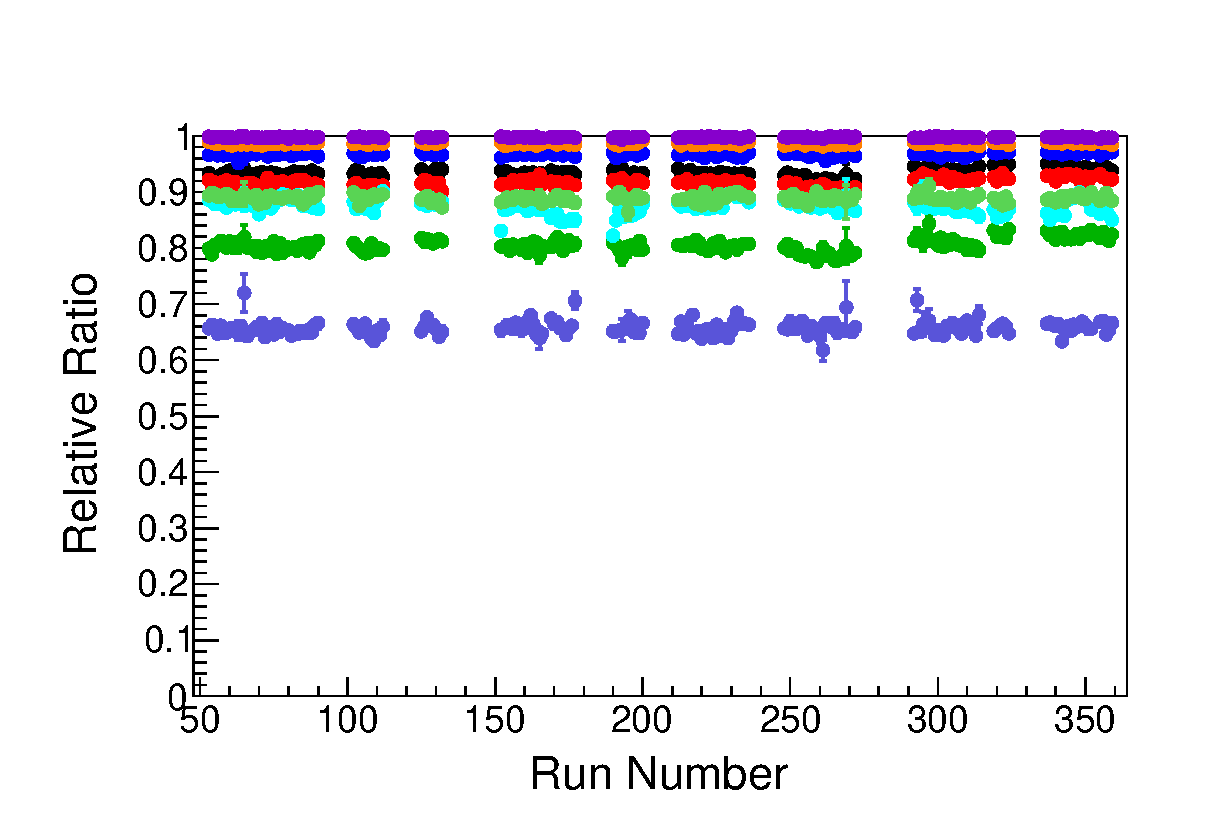
\includegraphics[width=6cm]{../pic/Run78/BL/relative_ratio.eps}
    \end{minipage}

    \begin{minipage}{0.5\hsize}
      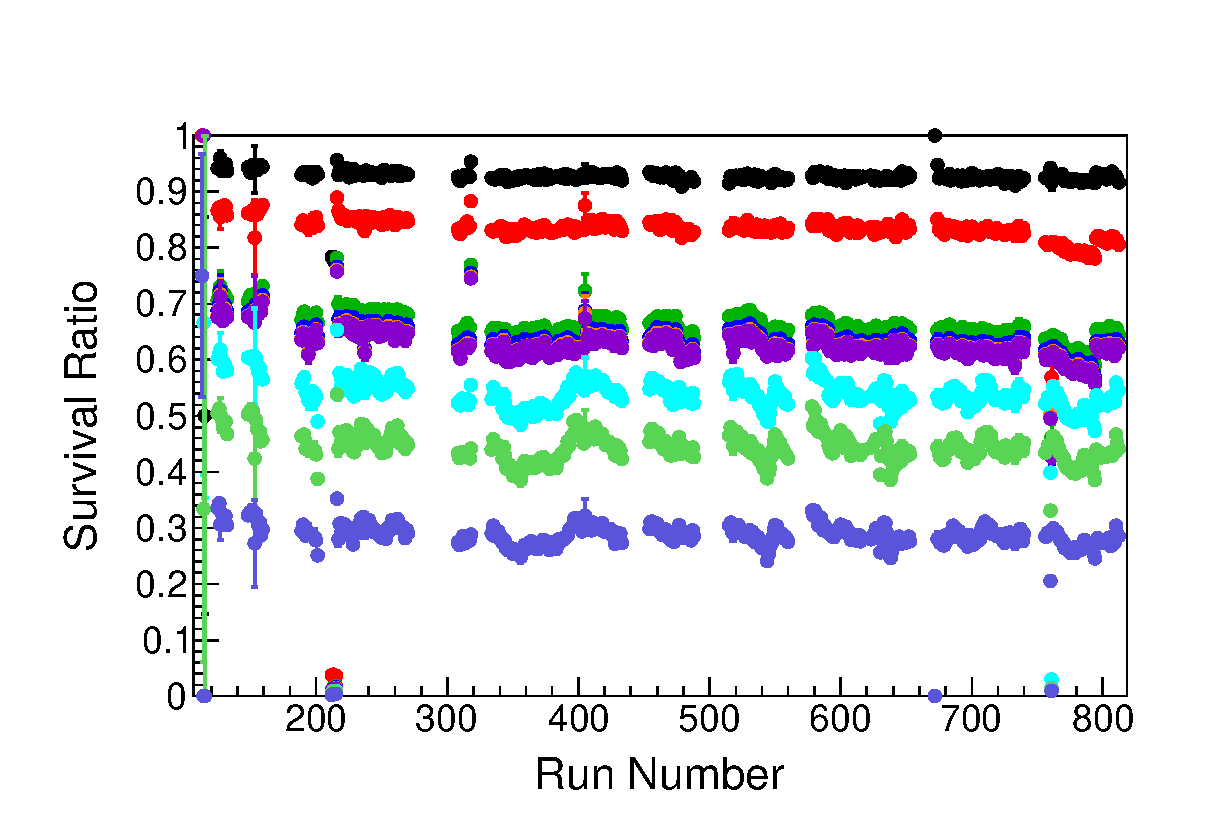
\includegraphics[width=6cm]{../pic/Run78/BL/survival_ratio.eps}
    \end{minipage}
  \end{tabular}
  \caption{
    Left and right figure indicates run dependence of relative and survival ratio in MR Run78, respectively.
    Relative ratio means ratio against before condition.
    Survival ratio means ratio from all K/f trigger events.
  }
  \label{fig:Kf_ratio}
\end{figure}

\begin{figure}[htbp]
  \centering
  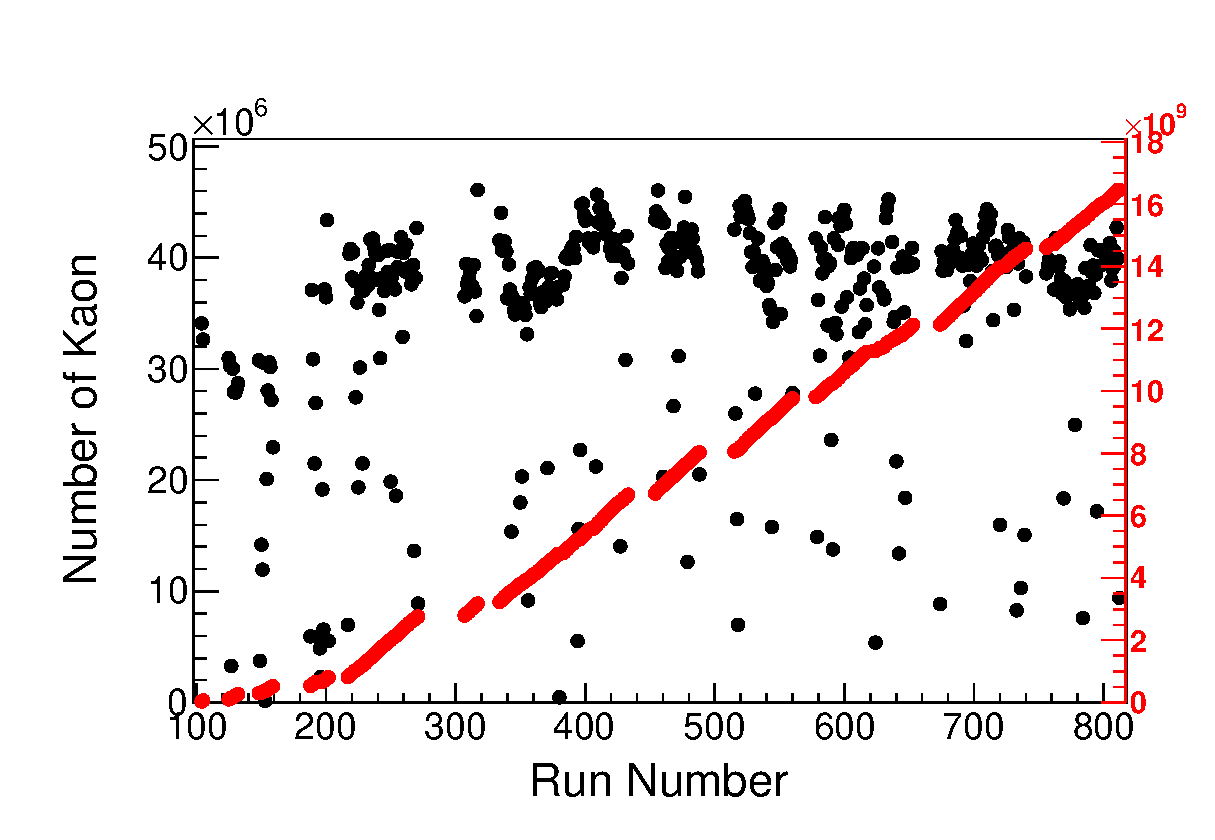
\includegraphics[width=8cm]{../pic/Run78/BL/Knum.eps}
  \caption{
    This figure shows kaon number irradiated on the liquid-$D_2$ target.
  }
  \label{fig:knum}
\end{figure}


The number of kaons irradiated to the liquid deuterium target is determined by multiplying the number of kaons counted by the scaler by the percentage left by the conditions imposed so far.
An estimate of the irradiated kaon beam is made for each operation and summed.

The selection of the beam actual through the liquid deuterium target takes place in the following order.

\begin{enumerate}
\item T0 1hit selection
\item T0-BHD TOF kaon selection
\item BLC1 1track selection
\item BLC2 1track selection
\item D5 momentum reconstruction
\item D5 and BHD matching selection
\item BPC 1track selection
\item BLC2 and BPC connection
\item Beam on target at FF
\end{enumerate}

These selections for each run are shown in Fig.\ref{fig:Kf_ratio}.
The right figure shows the ratio of the selection to the previous conditions, and the left figure shows the ratio of the remaining events to all unbaised kaon triggers.
